\documentclass[xetex,mathserif,serif]{beamer}
\usepackage{polyglossia}
\setdefaultlanguage[babelshorthands=true]{russian}
\usepackage{minted}
\usepackage{tabu}

\useoutertheme{infolines}

\usepackage{fontspec}
\setmainfont{FreeSans}
\newfontfamily{\russianfonttt}{FreeSans}

\usepackage{textpos}
\setlength{\TPHorizModule}{1cm}
\setlength{\TPVertModule}{1cm}

\definecolor{links}{HTML}{2A1B81}
\hypersetup{colorlinks,linkcolor=,urlcolor=links}

\tabulinesep=1.2mm

\title{Занятие 12: тестирование}
\author[Юрий Литвинов]{Юрий Литвинов\\\small{\textcolor{gray}{yurii.litvinov@gmail.com}}}
\date{11.10.2018}

\newcommand{\todo}[1] {
	\begin{center}\textcolor{red}{TODO: #1}\end{center}
}

\newcommand{\DownArrow} {
	\hspace{2cm}\begin{LARGE}$\downarrow$\end{LARGE}
}

\newcommand{\attribution}[1] {
	\begin{flushright}\begin{scriptsize}\textcolor{gray}{\textcopyright\; #1}\end{scriptsize}\end{flushright}
}

\begin{document}

	\frame{\titlepage}

	\section{Пример}

	\begin{frame}
		\frametitle{Пример}
		Консольный калькулятор, складывающий два двузначных числа
		\begin{itemize}
			\item Называется adder
			\item Ввод числа заканчивается нажатием на \textit{Enter}
			\item Программа должна вывести сумму после ввода второго числа
		\end{itemize}
		\begin{textblock}{5}(7,2)
			\attribution{C. Kaner, Testing Computer Software}
		\end{textblock}
	\end{frame}

	\begin{frame}
		\frametitle{Смоук-тест}
		\begin{center}
			\begin{tabu} {| X[0.6 l p] | X[1 l p] |}
				\tabucline-
				\everyrow{\tabucline-}
				\textbf{Что делаем}                             & \textbf{Что происходит}                                                            \\
				Вводим \textit{adder} и жмём на \textit{Enter}  & Экран мигает, внизу появляется знак вопроса                                        \\
				Нажимаем 2                                      & За знаком вопроса появляется цифра 2                                               \\
				Нажимаем \textit{Enter}                         & В следующей строке появляется знак вопроса                                         \\
				Нажимаем 3                                      & За вторым знаком вопроса появляется цифра 3                                        \\
				Нажимаем \textit{Enter}                         & В третьей строке появляется 5, несколькими строками ниже --- ещё один знак вопроса
			\end{tabu}
		\end{center}
	\end{frame}

	\begin{frame}
		\frametitle{Выявленные проблемы}
		\begin{itemize}
			\item Нет названия программы на экране, может, мы запустили не то
			\item Нет никаких инструкций, пользователь без идей, что делать
			\item Непонятно, как выйти
			\item Число 5 выведено слева от слагаемых, а не под ними
		\end{itemize}
	\end{frame}

	\begin{frame}
		\frametitle{План дальнейших тестов}
		\begin{scriptsize}
			\begin{center}
				\begin{tabu} {| X[2 l p] | X[2 l p] | X[7 l p] |}
					\tabucline-
					\everyrow{\tabucline-}
					\textbf{Ввод}  & \textbf{Ожидаемый результат}  & \textbf{Замечания}                                                      \\
					99 + 99        & 198                           & Пара наибольших допустимых чисел                                        \\
					-99 + -99      & -198                          & Отрицательные числа, почему нет?                                        \\
					99 + -14       & 85                            & Большое первое число может влиять на интерпретацию второго              \\
					-38 + 99       & 61                            & Отрицательное плюс положительное                                        \\
					56 + 99        & 155                           & Большое второе число может повлиять на интерпретацию первого            \\
					9 + 9          & 18                            & Два наибольших числа из одной цифры                                     \\
					0 + 0          & 0                             & Программы часто не работают на нулях                                    \\
					0 + 23         & 23                            & 0 --- подозрительная штука, его надо проверить и как первое слагаемое,  \\
					-78 + 0        & -78                           & и как второе
				\end{tabu}
			\end{center}
		\end{scriptsize}
	\end{frame}

	\begin{frame}
		\frametitle{План дальнейших тестов (2)}
		\begin{scriptsize}
			\begin{center}
				\begin{tabu} {| X[2 l p] | X[7 l p] |}
					\tabucline-
					\everyrow{\tabucline-}
					\textbf{Ввод}                   & \textbf{Замечания}                                                 \\
					100 + 100                       & Поведение сразу за диапазоном допустимых значений                  \\
					\textit{Enter} + \textit{Enter} & Что будет, если данные не вводить вообще                           \\
					123456 + 0                      & Введём побольше цифр                                               \\
					1.2 + 5                         & Вещественные числа, пользователь может решить, что так можно       \\
					A + b                           & Недопустимые символы, что будет?                                   \\
					\item{Ctrl-A, Ctrl-D, F1, Esc}  & Управляющие клавиши часто источник проблем в консольных программах \\
				\end{tabu}
			\end{center}
		\end{scriptsize}
	\end{frame}

	\begin{frame}
		\frametitle{Ещё больше тестов!}
		\begin{itemize}
			\item Внутреннее хранение данных --- двузначные числа могут хранить в \textbf{byte}
			\begin{itemize}
				\item 99 + 99, этот случай покрыли
			\end{itemize}
			\item Кодовая страница ввода: символы '/', '0', '9' и ':'
			\begin{itemize}
				\item Программист может напутать со строгостью неравенства при проверке
				\item Не надо вводить A + b, достаточно граничные символы
			\end{itemize}
		\end{itemize}
	\end{frame}

	\begin{frame}
		\frametitle{Rules of thumb}
		\begin{itemize}
			\item Отдельный багрепорт по каждому багу
			\item Если от двух тестов ожидается один и тот же результат, нужен только один
			\begin{itemize}
				\item Факторизация пространства состояний необходима
				\begin{itemize}
					\item Но невозможна --- мы не знаем, как оно устроено внутри
				\end{itemize}
				\item Из класса тестов выбирается тот, на котором баг вероятнее всего
			\end{itemize}
			\item Всегда надо записывать, что делали и что происходит
			\item Проверяйте граничные условия
			\item Большая часть тестов ошибок не выявит
			\item Подсистемы обработки ошибок впиливают в последнюю очередь, поэтому они часто полны багов
		\end{itemize}
	\end{frame}

	\section{Цель тестирования}

	\begin{frame}
		\frametitle{Жизнь тестировщика --- боль}
		\begin{itemize}
			\item Самое важное:
			\begin{itemize}
				\item Любая программа содержит ошибки
				\item Если программа ошибок не содержит, их содержит спецификация, которую она реализует
				\item Если ни программа, ни спецификация ошибок не содержит, такая программа даром никому не нужна
			\end{itemize}
			\item Полностью протестировать программу невозможно
			\begin{itemize}
				\item Комбинаторный взрыв входных данных
				\item Экспоненциальное количество путей исполнения
				\item Баги, связанные с асинхронностью и многопоточностью
				\item Баги, связанные с пользовательским интерфейсом
			\end{itemize}
			\item Формально доказать корректность программы невозможно
		\end{itemize}
	\end{frame}

	\begin{frame}
		\frametitle{Пример}
		\begin{itemize}
			\item Телефон --- конечный автомат из 6 состояний
			\begin{itemize}
				\item 1 --- телефон молчит, при входящем вызове (состояние 2) абонент снимает трубку (состояние 3) или
					звонящий вешает трубку (состояние 5). Ответив на звонок, абонент может нажать \textit{Hold} (состояние 4)
					или повесить трубку (состояние 5), при этом после нажатия на \textit{Hold} можно ответить на другой звонок
					(состояние 6)
			\end{itemize}
			\item По нажатию \textit{Hold} телефон помещает данные в стек
			\item Если звонящий вешает трубку, пока его линия в \textit{Hold}, данные не снимались со стека
			\item По возврату в состояние 1 стек очищается
			\item Глубина стека --- 30. Упс.
		\end{itemize}
	\end{frame}

	\begin{frame}
		\frametitle{Информация к размышлению}
		\begin{itemize}
			\item Программа из сотни строк может иметь $10^{18}$ путей исполнения
			\begin{itemize}
				\item Времени жизни вселенной не хватило бы, чтобы их покрыть
			\end{itemize}
			\item После передачи на тестирование в программах в среднем от 1 до 3 ошибок на 100 строк кода
			\item В процессе разработки --- 1.5 ошибок на 1 строку кода (!)
			\item Если для исправления ошибки надо изменить не более 10 операторов, с первого раза это делают правильно в 50\% случаев
			\item Если для исправления ошибки надо изменить не более 50 операторов, с первого раза это делают правильно в 20\% случаев
		\end{itemize}
	\end{frame}

	\begin{frame}
		\frametitle{Цель тестирования}
		\begin{itemize}
			\item Цель тестирования --- сделать так, чтобы ошибки исправили
			\item Основная задача тестировщика --- выявить ошибки
			\begin{itemize}
				\item И ``продать'' их программистам и руководству
			\end{itemize}
			\item Тест, который не выявил ошибку --- пустая трата времени
			\item Чем раньше будет выявлена ошибка, тем проще её исправить
		\end{itemize}
	\end{frame}

	\section{Виды тестирования}

	\begin{frame}
		\frametitle{Тестирование требований}
		\begin{itemize}
			\item Выполняется на этапе планирования
			\item Цели:
			\begin{itemize}
				\item Адекватность требований
				\item Полнота, непротиворечивость и т.д.
				\item Выполнимость, рентабельность
				\item Возможность тестирования
			\end{itemize}
			\item Способы:
			\begin{itemize}
				\item Обзор аналогов
				\item ``Дискуссионные группы''
				\item Исследование объекта автоматизации
			\end{itemize}
		\end{itemize}
	\end{frame}

	\begin{frame}
		\frametitle{Тестирование архитектуры}
		\begin{itemize}
			\item Выполняется на этапе проектирования
			\item Цели:
			\begin{itemize}
				\item Проверка соответствия требованиям
				\item Проверка ожидаемых качеств
				\item Проверка полноты и реалистичности
				\item Проверка подсистемы обработки ошибок
			\end{itemize}
			\item Методы:
			\begin{itemize}
				\item Ревью
				\item Формальный анализ архитектуры
			\end{itemize}
		\end{itemize}
	\end{frame}

	\begin{frame}
		\frametitle{Тестирование ``белого ящика'', юнит-тесты}
		\begin{itemize}
			\item Coverage
			\begin{itemize}
				\item Покрытие строк кода --- самый слабый критерий
				\item Покрытие путей исполнения --- тоже не полный
				\item Покрытие всех составляющих каждого условия --- символьное исполнение?
				\item Всё равно особо не поможет (var x = y / z;)
			\end{itemize}
			\item Стратегии тестирования:
			\begin{itemize}
				\item ``Снизу вверх'' --- юнит-тесты
				\item ``Сверху вниз'' --- интеграционные тесты + моки
			\end{itemize}
			\item Статическое тестирование
			\item Мутационное тестирование
			\item Регрессионное тестирование
		\end{itemize}
	\end{frame}

	\begin{frame}
		\frametitle{Тестирование ``чёрного ящика''}
		\begin{itemize}
			\item Квалификационное тестирование (смоук-тест)
			\begin{itemize}
				\item Квалификационные тесты имеет смысл опубликовать
			\end{itemize}
			\item Оценочное тестирование
			\item Функциональное тестирование --- проверка на соответствие спецификации
			\item Тестирование целостности --- проверка на соответствие пользовательской документации
			\item Бета-тестирование
			\item Тестирование инсталлятора
			\item Приёмка и сертификация
			\item ...
		\end{itemize}
	\end{frame}

	\begin{frame}
		\frametitle{Примеры видов тестов ``чёрного ящика''}
		\begin{itemize}
			\item Сверка со спецификацией
			\item Лабораторные испытания на группе потенциальных пользователей
			\item Тесты на эргономичность
			\item Тесты на граничные условия
			\item Тесты на производительность
			\item Тесты на переходы между состояниями
			\item Тесты на асинхронное взаимодействие
			\item Эксплуатация в реальном режиме
			\item Нагрузочные тесты
			\item Тесты на обработку ошибок
			\item Тесты на защиту от несанкционированного доступа
			\item Тесты на совместимость импорта/экспорта и программную совместимость
			\item Тесты на аппаратные конфигурации
			\item Адаптационное тестирование
		\end{itemize}
	\end{frame}

	\section{Ошибки}

	\begin{frame}
		\frametitle{Что такое ``Ошибка''}
		\begin{itemize}
			\item Качество ПО определяется:
			\begin{itemize}
				\item Возможностями, которыми оно понравится пользователю
				\item Недостатками, которые вынудят пользователя купить другое ПО
			\end{itemize}
			\item \textbf{Соответствие спецификации, качество кода и т.д. --- не качество!}
			\item Понятие ``ошибка'' субъективно
		\end{itemize}
	\end{frame}

	\begin{frame}
		\frametitle{Категории ошибок}
		\begin{itemize}
			\item Ошибки пользовательского интерфейса
			\begin{itemize}
				\item Функциональность --- программа не делает того, что от неё ожидает пользователь
				\begin{itemize}
					\item Пользователей много и все ожидают что-то своё
				\end{itemize}
				\item Взаимодействие с пользователем
				\item Структура интерфейса
				\item Пропущенная функциональность
				\item Производительность
				\item Выходные данные
			\end{itemize}
		\end{itemize}
	\end{frame}

	\begin{frame}
		\frametitle{Категории ошибок (2)}
		\begin{itemize}
			\item Обработка ошибок
			\item Обработка граничных условий
			\item Ошибки вычислений
			\item Ошибки инициализации и первого запуска
			\item Ошибки управления потоком
			\item Ошибки хранения, передачи или интерпретации данных
			\item Гонки
			\item Ошибки работы под нагрузкой
			\item Ошибки взаимодействия с аппаратным обеспечением			
		\end{itemize}
	\end{frame}

	\begin{frame}
		\frametitle{Категории ошибок (3)}
		\begin{itemize}
			\item Ошибки версионного контроля
			\item Ошибки документации
			\begin{itemize}
				\item Да, её тоже тестируют
				\begin{itemize}
					\item Более того, надо внимательно проверять вообще всё, что ``кладётся в коробку''
				\end{itemize}
			\end{itemize}
			\item Ошибки тестирования
			\begin{itemize}
				\item Тесты тоже содержат код, следовательно, ошибки
			\end{itemize}
		\end{itemize}
	\end{frame}

	\section{Test Plan}

	\begin{frame}
		\frametitle{Test plan}
		\begin{itemize}
			\item План тестирования --- формальный документ, описывающий, что, как и когда надо проверить
			\item Нужен, чтобы:
			\begin{itemize}
				\item Ничего не забыть и не пропустить
				\item Проанализировать программу и выбрать лучшие тесты
				\item Обеспечить взаимодействие между членами команды
				\item Выполнить оценку трудозатрат
				\item Скорректировать спецификацию и архитектуру системы
			\end{itemize}
			\item Стандарты IEEE-829 и IEEE-29119
			\begin{itemize}
				\item Как правило, не нужны
				\item План полезен настолько, насколько он помогает организации тестирования и поиску ошибок
			\end{itemize}
		\end{itemize}
	\end{frame}

	\begin{frame}
		\frametitle{Какие тесты фиксировать в плане}
		\begin{itemize}
			\item Тестирование ``белого ящика'' часто оставляют программистам
			\item Что оно упускает:
			\begin{itemize}
				\item Ошибки, связанные со временем --- гонки, асинхронность
				\item Особые стечения данных
				\begin{center}
					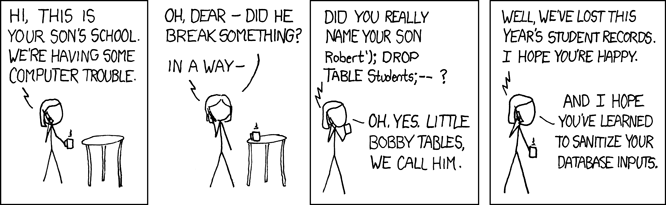
\includegraphics[width=0.7\textwidth]{xkcd.png}
					\attribution{xkcd.com}
				\end{center}
				\item Всё, что относится к UI
				\item Ошибки, связанные с конфигурацией и совместимостью
				\item Аппаратные ошибки
			\end{itemize}
		\end{itemize}
	\end{frame}

	\begin{frame}
		\frametitle{Составляющие тест-плана}
		\begin{center}
			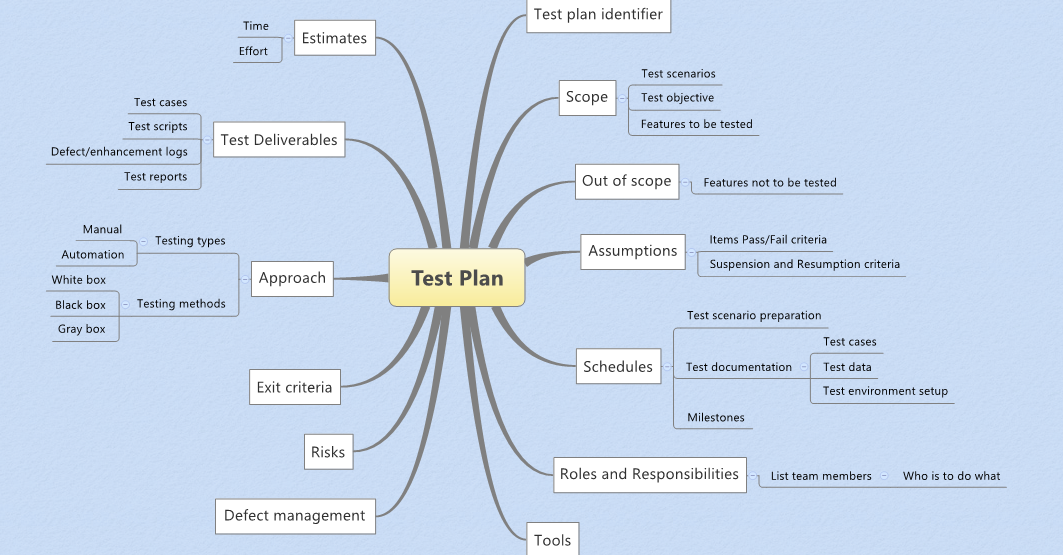
\includegraphics[width=\textwidth]{testPlan.png}
			\attribution{http://darshandeshmukh.blogspot.com}
		\end{center}
	\end{frame}

	\begin{frame}
		\frametitle{Как писать тест-план}
		\begin{enumerate}
			\item Проанализировать продукт
			\begin{itemize}
				\item Список фич
				\item Список экранов
				\item Список файлов
			\end{itemize}
			\item Определиться со стратегией тестирования
			\item Выписать типы ошибок, на которые хотим вообще проверять
			\item Определиться с тем, что мы считаем ок, а что не ок
			\item Прикинуть способы проверки штук из п. 1 на ошибки из п. 3
			\item Оценить трудоёмкость
			\item Посмотреть, нельзя ли сэкономить (урезанием функциональности, например)
			\item Назначить ресурсы, составить календарный план
		\end{enumerate}
	\begin{footnotesize}См. \url{https://www.guru99.com/what-everybody-ought-to-know-about-test-planing.html}\end{footnotesize}
	\end{frame}

	\section{Задача}

	\begin{frame}
		\frametitle{Задача}
		\begin{itemize}
			\item Написать план тестирования для своего проекта
			\begin{itemize}
				\item Что тестируем
				\begin{itemize}
					\item Перечислить совместимые ОС, оборудование, окружение
				\end{itemize}
				\item На какие типы ошибок проверяем
				\item Какими методами тестирования пользуемся
				\item Условия прекращения и продолжения тестирования
				\item Оценки трудоёмкости и календарный план тестов
			\end{itemize}
			\item Каждому члену команды выбрать один тестовый случай и написать тестовый сценарий
			\begin{itemize}
				\item Summary теста
				\item Последовательность шагов
				\begin{itemize}
					\item Что делать
					\item Что ожидается получить
				\end{itemize}
			\end{itemize}
			\item Выложить на вики проекта на гитхабе
		\end{itemize}
	\end{frame}

\end{document}
